
\section{Bevezetés}

Ide jön a bevezetés...\cite{wiley_ims}

\subsection{Motiváció}

Napjaink infokommunikációs hálózatainak fejlődési tendenciája azt mutatja, hogy az egymástól elszigetelt,
különálló szolgáltató hálózatok helyett egy konvergált, egységes hálózat van kialakulóban. Egységes hálózaton azt értem, hogy a felhasználók azonos módon érhetik el a szolgáltatásokat, függetlenül attól, hogy éppen milyen hálózatról, milyen eszközzel -- mobil vagy fix -- kívánják ezt megtenni. Ehhez egyrészt az szükséges, hogy a fix és a mobil hálózatok konvergenciája megvalósuljon (fixed-mobile convergence), másrészt a szolgáltatások azonos hálózatra történő konvergeciájára is szükség van (multiple play). Utóbbi azt jelenti, hogy egy szolgáltató ugyanazon a hálózaton képes különböző szolgáltatásokat nyújtani az előfizetőknek. Itt jut szerephez az IMS (IP Multimedia Subsystem). Az IMS-ről részletesebben a \ref{sec:ims}.~fejezetben lesz szó.

Korunkban egyre többen használnak különféle elektronikus kommunikációs formákat, különféle környezetben, különböző eszközökkel. Ezek az eszközök jellemzően más-más módon kommunikálnak egymással, amely sok esetben jelentős kompatibilitási problémákhoz vezet.

\subsection{Célkitűzés}

A feladat célkitűzése egy olyan rendszer megalkotása az IMS rendszerben, melynek
segítségével a felhasználóknak lehetősége nyílik multimédia üzenet küldésére felhasználók egy megadott csoportjának. Fontos szempont az is, hogy ha egy felhasználó az üzenetküldés idejében éppen nem kapcsolódik a hálózathoz, akkor is megkapja a neki szánt üzeneteket. Ezt a funkciót késleltetett üzenettovábbításnak nevezik.

\subsection{Az IP Multimédia Alrendszer}
\label{sec:ims}

Az IMS jelentős lépés az ``all-IP'' hálózati architektúra felé. Egységes jelzési hálózatot nyújt az eszközöknek, amely jel\-zés\-há\-ló\-zat különválik a tartalom átvitelért felelős hálózattól, ezáltal a két hálózaton használt kommunikációs formák teljesen függetlenek lesznek egymástól. A következő generációs hálózatok (Next Generation Network - NGN) egy lehetséges jelzéssíkjaként az IMS célja a cellás és IP hálózati multimédia szolgáltatások fúziója. Az IMS-ben jelzési protokollnak a  SIP (Session Initiaton Protocol) protokollt választották. A SIP egy alkalmazás rétegbeli protokoll, amely lehetővé teszi multimédia kapcsolatok felépítését, módosítását, befejezését IP (Internet Protocol) hálózatok felett. 

\subsubsection{A hálózat főbb funkcionális egységei}

Az IMS hálózat három rétegre bontható: a maghálózatra, a maghálózat felett elhelyezkedő egységesen elérhető szolgáltatásokra, illetve a hozzáférési hálózatokra.

\begin{figure}[htbp]
\center
\resizebox{11cm}{!}{
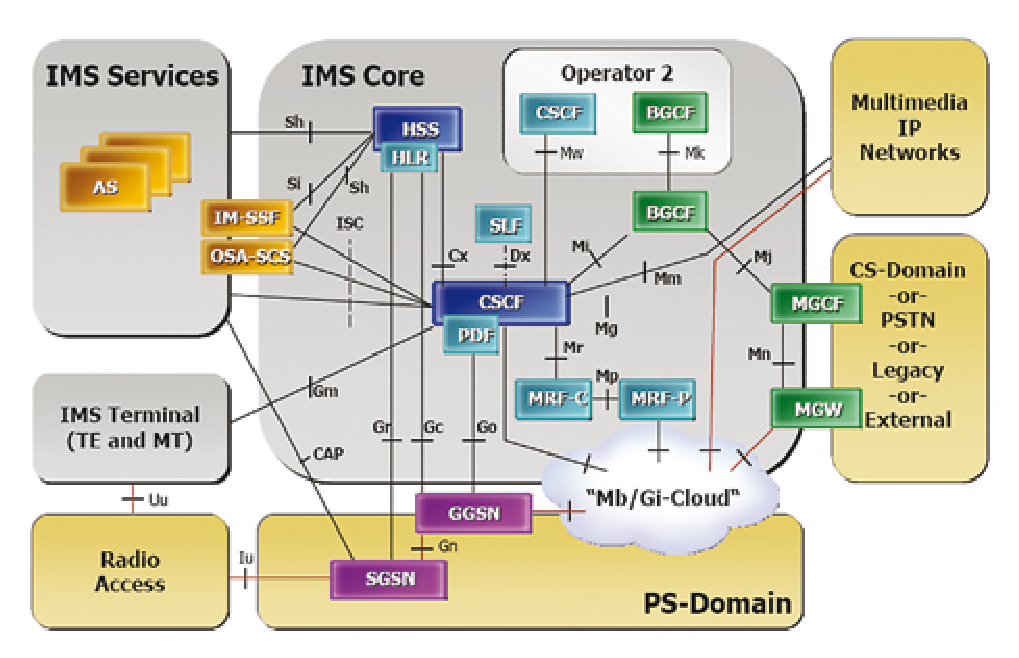
\includegraphics{img/ims-network.eps}}
\caption{Az IMS hálózat felépítése~\cite{ims_figure} }
\label{fig:model}
\end{figure}


A maghálózat fő adatbázisa a \emph{Home Subscriber Server} (HSS), amely többek között olyan felhasználó-specifikus információkat tartalmaz, mint a hitelesítő információk, előfizetői adatok, felhasználói profilok, tartózkodási hely információk, stb. Az IMS hálózat tartalmazhat több HSS-t is, ekkor viszont szükség van egy \emph{Subscription Locator Function} (SLF) nevű egységre is. Az SLF tartalmazza, hogy melyik felhasználó adatai melyik HSS-ben vannak tárolva.

A maghálózat központi egysége a \emph{Call/Session Control Function} (CSCF), amely tulajdonképpen egy SIP szerver. Feladatai közé tartozik többek között a SIP üzenetek feldolgozása, a kapcsolatok kezelése. Három típusa van:
\begin{itemize}
\item A \emph{P-CSCF} (Proxy-CSCF) a jelzés síkban belépési pont a terminál és az IMS hálózat között, lényegében egy bemenő/kimenő SIP proxy szerver. Feladatai közé tartozik a felhasználók hitelesítése, a SIP üzenetek helyességének ellenőrzése. A felhasználóktól jövő vagy a nekik szánt üzeneteket tömörítheti. Utóbbi a cellás hálózatokban előnyös, ahol a rádiós erőforrás sávszélessége szűkös. Számlázási információkat is generálhat. Ezen kívül a P-CSCF tartalmazhat Policy Decision Function-t (PDF), amely a média síkban kezeli az erőforrásokat, ezáltal megfelelő szolgáltatás minőség (Quality of Service - QoS) biztosítható vele. Egy IMS hálózatban általában több P-CSCF van, ami a skálázhatóság és megbízhatóság szempontjából lényeges.
\item Az \emph{I-CSCF} (Interrogating-CSCF) az adminisztratív tartomány határán található SIP proxy szerver. Címe megtalálható a tartomány DNS-ében (Domain Name System). Ha a felhasználói terminál idegen hálózatban tartózkodik (például roaming esetén), ahol a szintén idegen hálózatban található egyik Proxy-CSCF-hez kapcsolódik, akkor a P-CSCF a DNS alapján megkeresi a felhasználó otthoni hálózatához tartozó I-CSCF-et, és a kliens felől érkező jelzés üzeneteket továbbküldi oda továbbítja. Az I-CSCF-nek interfésze van mind az SLF, mind a HSS felé. Ha az I-CSCF jelzés üzenetet kap, akkor az SLF-től és a HSS-től lekérdezi a felhasználót kiszolgáló S-CSCF címét, majd az üzenetet továbbítja a kapott címre. A hálózatban több I-CSCF van jelen a skálázhatóság és a megbízhatóság miatt.
\item Az \emph{S-CSCF} (Serving-CSCF) a jelzés sík központi eleme. Mindig a felhasználó otthoni hálózatában helyezkedik el. Feladatai közé tartozik a kapcsolatkezelés, illetve SIP registrar-ként is működik. Ez végzi a felhasználók tartózkodási helyének címe (a terminál IP címe, ahol éppen tartózkodik) illetve a SIP címe (Public User Identity) közötti kötést. A HSS-től kéri le a felhasználók hitelesítő vektorait, profiljait. Utóbbiban van a triggerek halmaza, amelyből tudja, hogy melyik alkalmazás szervernek kell továbbítania a felhasználótól jövő SIP üzeneteket. A felhasználó regisztrációjáról értesíti a HSS-t, amelyben eltárolódik a felhasználó aktuális állapota. Egyik fő funkciója a SIP üzenetek útvonalválasztása. Címfordítást is végez, ha például a felhasználó telefonszámot tárcsáz SIP URI (Uniform Resource Identifier) helyett. Több S-CSCF lehet a hálózatban szintén a skálázhatóság és a redundancia végett.
\end{itemize}

A maghálózat feletti szolgáltatási réteg tartalmaz egy vagy több \emph{alkalmazás szer\-vert} (Application Server - AS), amely az elérhető szolgáltatásokat nyújtja. Az aktuális szolgáltatástól függően futhat SIP proxyként, vagy SIP User Agentként (SIP UA), mint végpont. Az S-CSCF-vel a SIP protokoll segítségével kommunikál.

Az IMS hálózatban jelen van egy vagy több \emph{MRF} (Media Resource Function), amelyek jelzés síkban MRF Controller-ből (MRFC), média síkban MRF Processor-ból (MRFP) állnak.  Az MRF az otthoni hálózatban a média forrása, a médiafolyamok átalakításáért, lejátszásáért felelős. Az MRFC SIP UA-ként viselkedik, H.248-as interfészen keresztül vezérli az MRFP erőforrásait.

A hálózat továbbá tartalmaz egy vagy több \emph{BGCF-t} (Breakout Gateway Control Function), amely alapvetően SIP szerver, és amely a telefonszám alapú út\-vo\-nal\-vá\-lasz\-tást végzi. Akkor használjuk, ha egy IMS terminál áramkörkapcsolt hálózatban, mint például PSTN-ben (Public Switched Telephone Network – nyilvános kapcsolt telefonhálózat) vagy PLMN-ben (Public Land Mobile Network, nyilvános földi mobil hálózat) végződő hívást kezdeményez.

Az áramkörkapcsolt hálózatok felé való átjárásért a \emph{PSTN Gateway} felelős, a\-mely három részből áll: egyrészt SGW-ből (Signalling Gateway), MGW-ből (Media Gateway), valamint MGCF-ből áll (Media Gateway Controller Function). Az SGW interfész alacsonyabb rétegbeli protokoll konverziót végez az áramkörkapcsolt hálózat jelzés síkja felé. Az MGW az áramkörkapcsolt hálózat média síkja felé nyújt kapcsolatódási pontot, Real-time Transport Protocol (RTP) felett küld és fogad IMS médiafolyamokat. Az MGCF a központi elem, tulajdonképpen egy állapotgép a PSTN gatewayben, feladata az MGW és SGW vezérlése.

\subsubsection{A felhasználók azonosítása}

A felhasználóknak egy vagy több publikus felhasználó azonosítójuk (Public User Identitities), és pontosan egy privát azonosítójuk van (Privat User Identity). A publikus azonosító lehet a SIP URI (Uniform Resource Identifier, RFC 3261~\cite{rfc3261}), vagy a TEL URI (RFC 3966~\cite{rfc3966}). Ezen publikus azonosítókat a tartomány operátora osztja ki, és ezeket használja az IMS hálózat az útvonalválasztás során. A privát azonosító nem TEL URI vagy SIP URI, hanem formailag követi a NAI alakot (Network Access Identifier, RFC 2486~\cite{rfc2486}). A privát azonosítókat csak hitelesítésre használják.

